\documentclass[]{article}

\usepackage[utf8]{inputenc}
\usepackage[T1]{fontenc}
\usepackage[frenchb]{babel}
\usepackage{amsmath,amsfonts,amssymb,amsthm}
\usepackage{graphicx}

\begin{document}

\paragraph{}Pour suivre le même principe que les diagrammes de séquence de la partie commune, seuls les diagrammes de séquences des cas d’utilisation ne se limitant pas à la création et la manipulation d’un objet instancié via l’API seront détaillés.

\begin{figure}[h!]
\hbox{
    \centering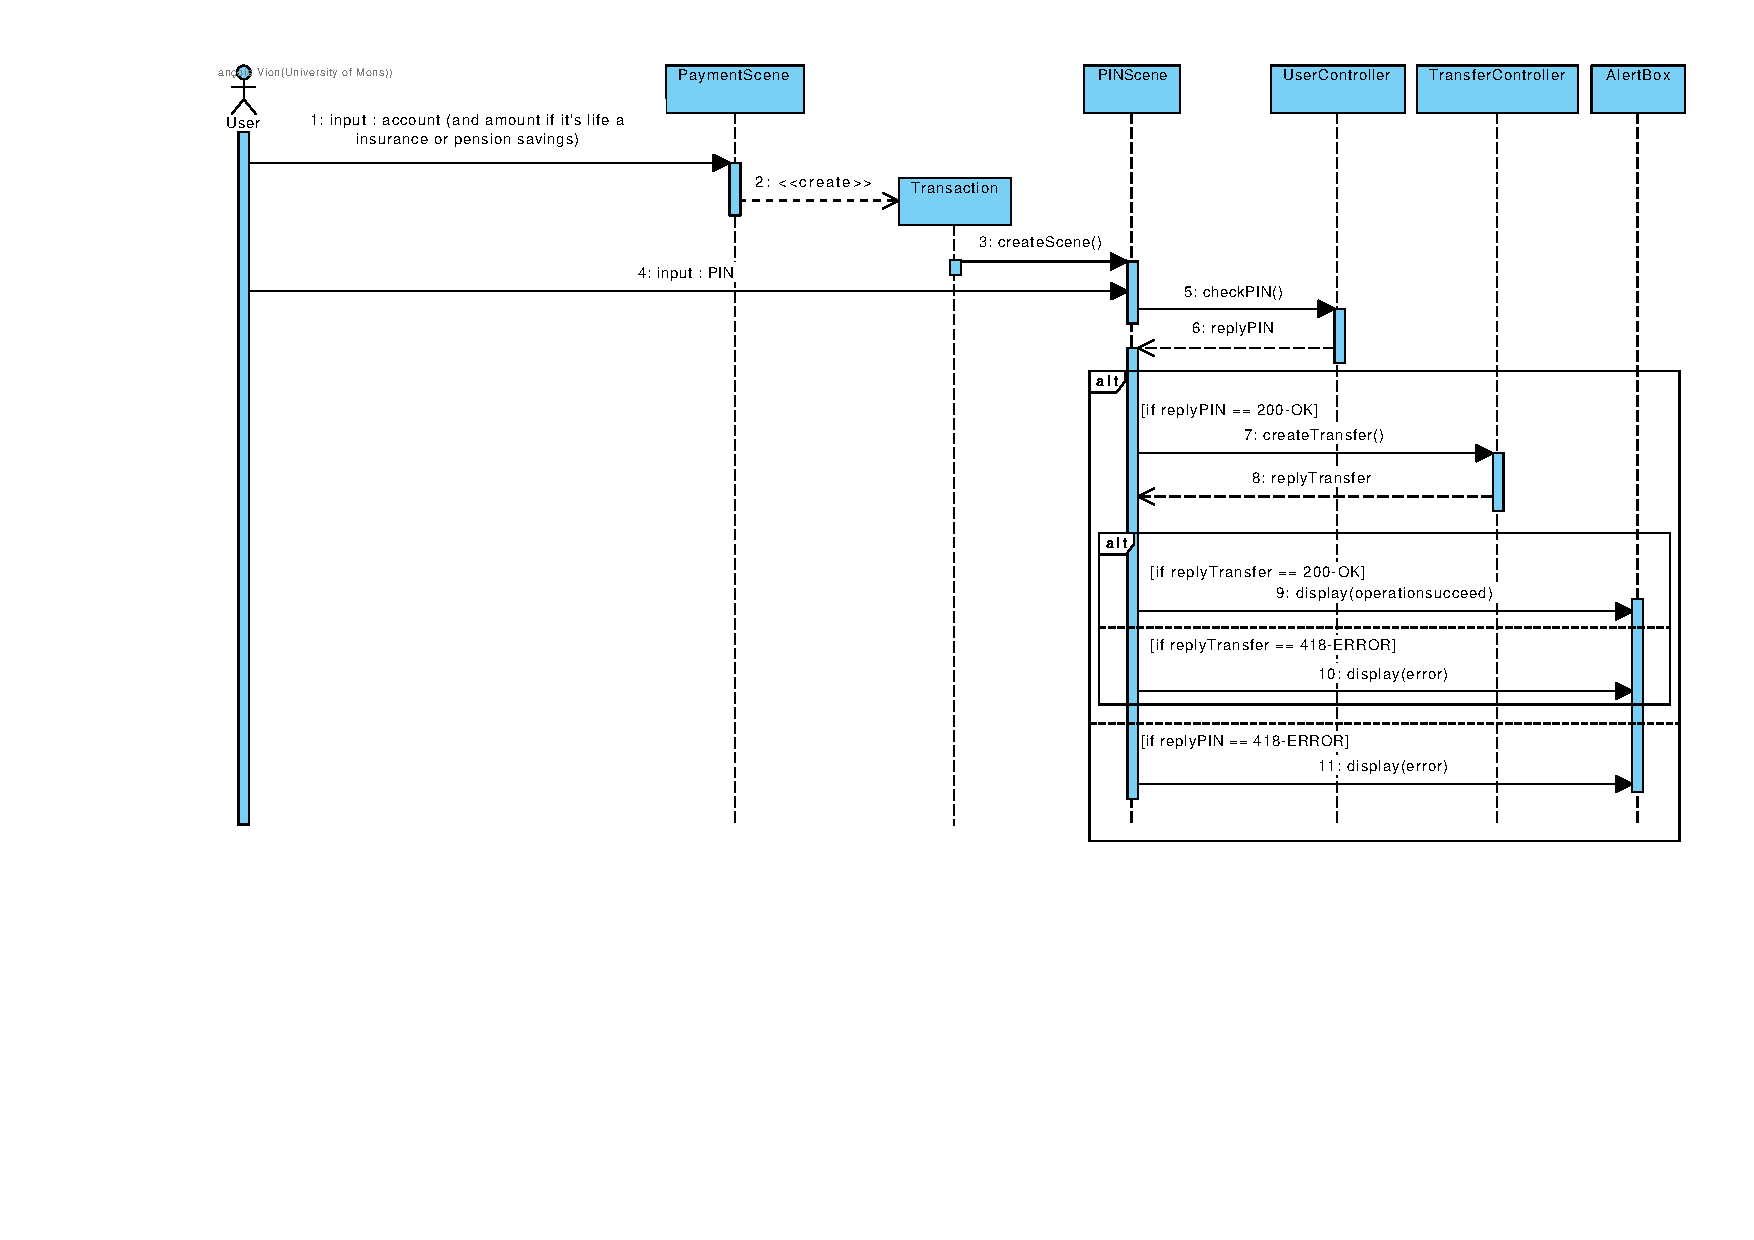
\includegraphics[width=\linewidth]{img/Payer la prime annuelle.pdf}
}
\caption{Diagramme de séquence du use case "Payer la prime annuelle"}
\end{figure}

\paragraph{} Pour payer la prime annuelle, le client rentre sur la scene le compte avec lequel il compte payer ainsi que le montant à payer s’il s’agit d’une assurance vie ou épargne pension (1). Un objet Transaction est créé (2). Celui-ci va créer la scene de confirmation avec le code PIN (3). Ensuite, l’utilisateur va rentrer son code PIN (4). Celui-ci sera vérifié via l’API (5) et elle renverra une réponse (6). Si cette réponse est 200-OK, alors on crée le transfert via l’API (7) qui renvoie une réponse (8). Si la réponse au transfert est bonne (200-OK), alors une fenêtre est affichée pour signaler que l’opération a bien été effectuée (9). Si l’une des 2 réponses est mauvaise (418-ERROR), on affiche une fenêtre qui signale qu’il y a eu une erreur (10 et 11).

\newpage

\begin{figure}[h!]
    \hbox{
        \centering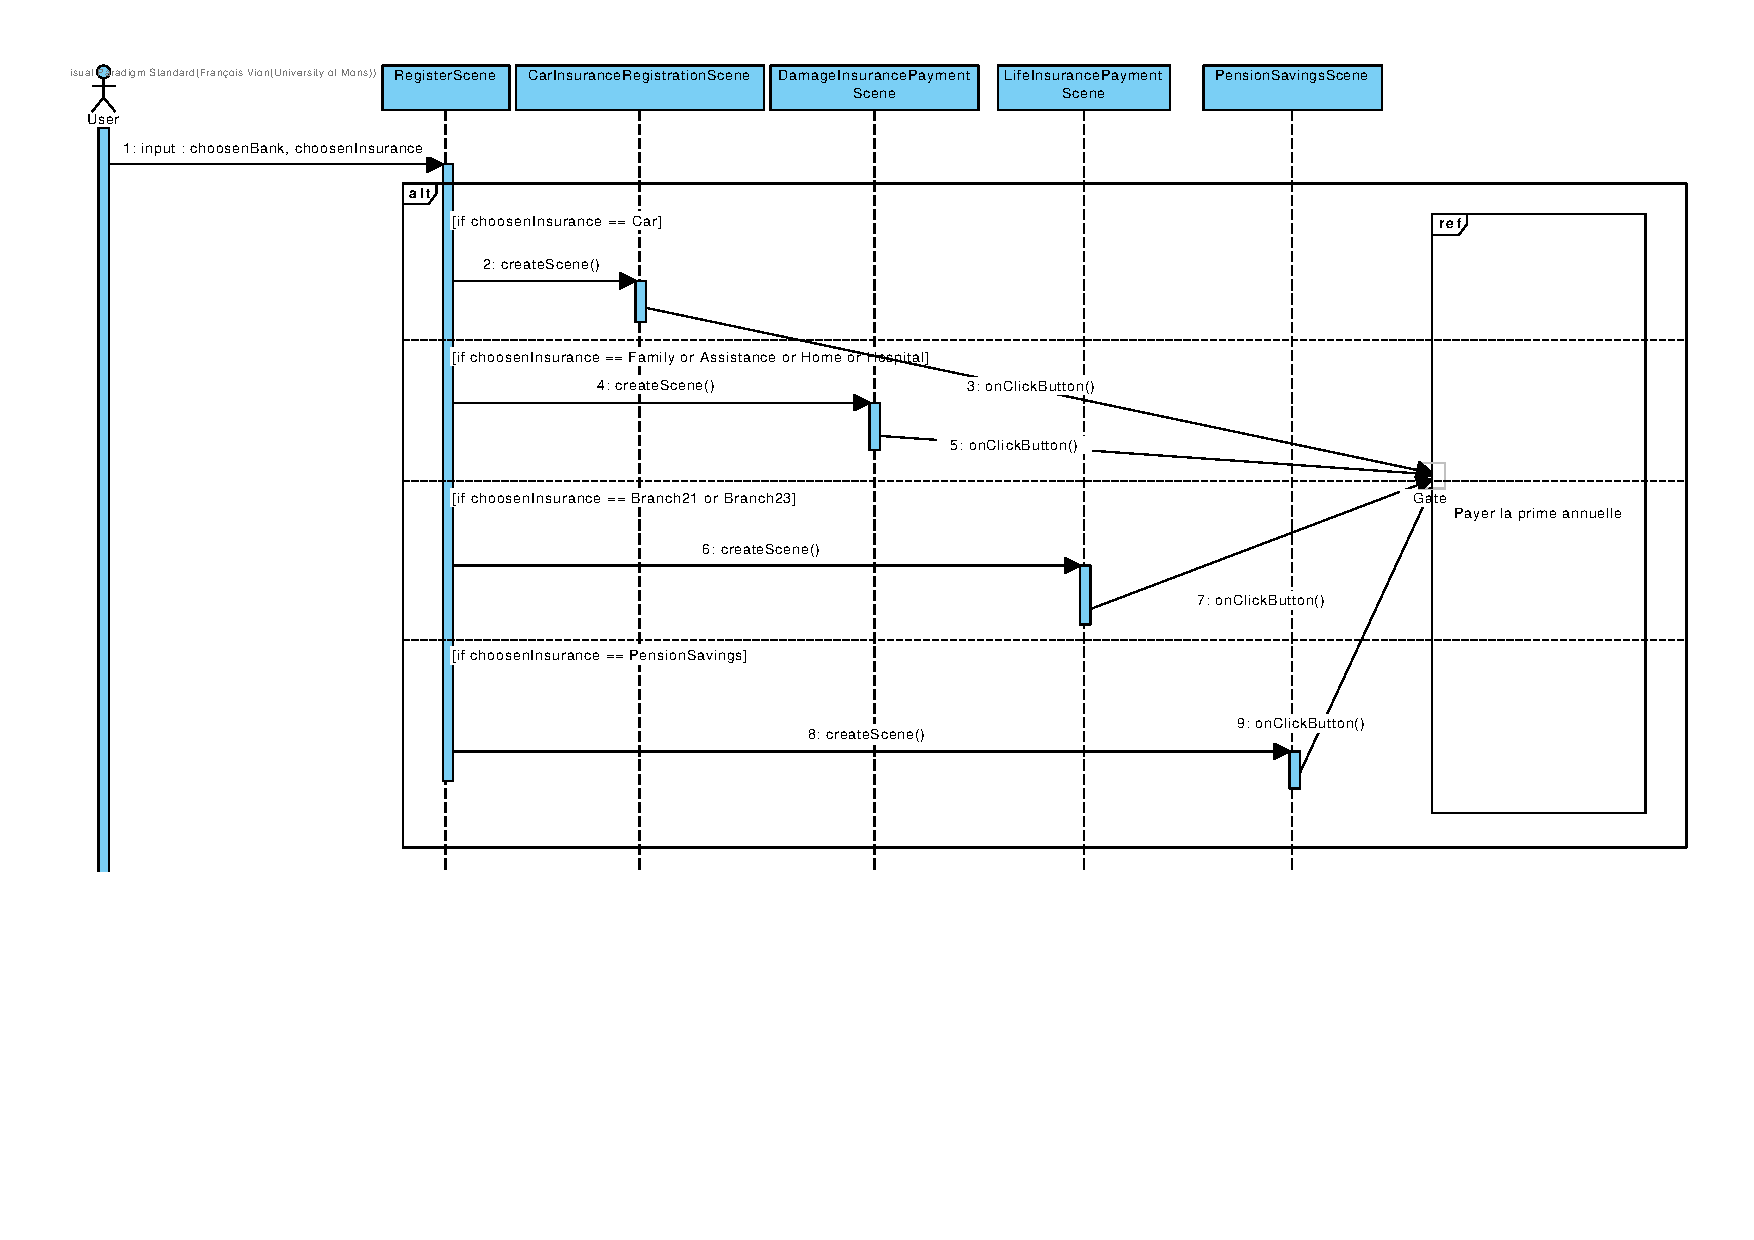
\includegraphics[width=\linewidth]{img/S'inscrire à une assurance.pdf}
    }
    \caption{Diagramme de séquence du use case "S'inscrire à une assurance"}
    \end{figure}

\paragraph{}S’inscrire à une assurance commence par le choix de banque et d’assurance par l’utilisateur (1). Ensuite, plusieurs cas se distinguent même s' ils fonctionnent de la même manière. Une scene correspondante au type d’assurance est créée (2, 4,6 et 8) et reprend les informations sur l’assurance choisie ainsi que le choix des options possibles dans le cas de l’assurance voiture. Enfin, en cliquant sur le bouton de la fenêtre, on accède à la fenêtre de payement afin de confirmer l’inscription (3,5,7 et 9). Le payement ne sera pas décrit car il s’agit exactement du cas cité précédemment dans le rapport.

\newpage

\begin{figure}[h!]
    \hbox{
        \centering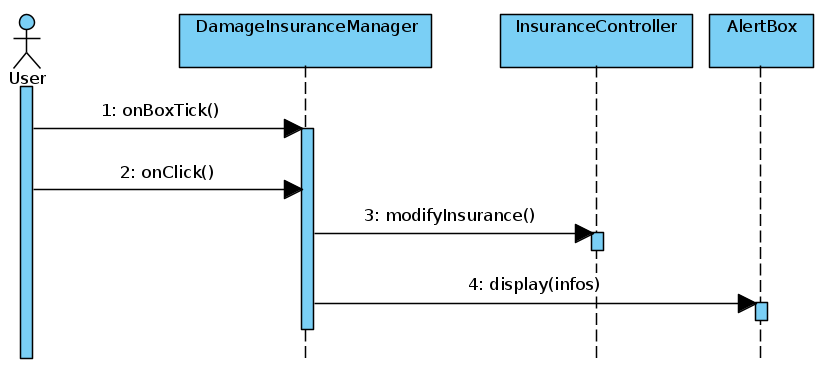
\includegraphics[width=\linewidth]{img/Modifier les paramètres d'une assurance.png}
    }
    \caption{Diagramme de séquence du use case "Modifier les paramètres d'une assurance"}
    \end{figure}

\paragraph{}Modifier les paramètres d’une assurance se fait via une scene avec des boutons “checkBox”. L’utilisateur commence par les cocher ou décocher (1) puis clique sur le bouton “save changes” (2). Une fois cela fait, la scene fait un appel à l’API pour modifier l’assurance dans la base de données (3). Enfin, une fenêtre reprenant les informations suite à la modification est affichée.

\newpage

\begin{figure}[h!]
    \hbox{
        \centering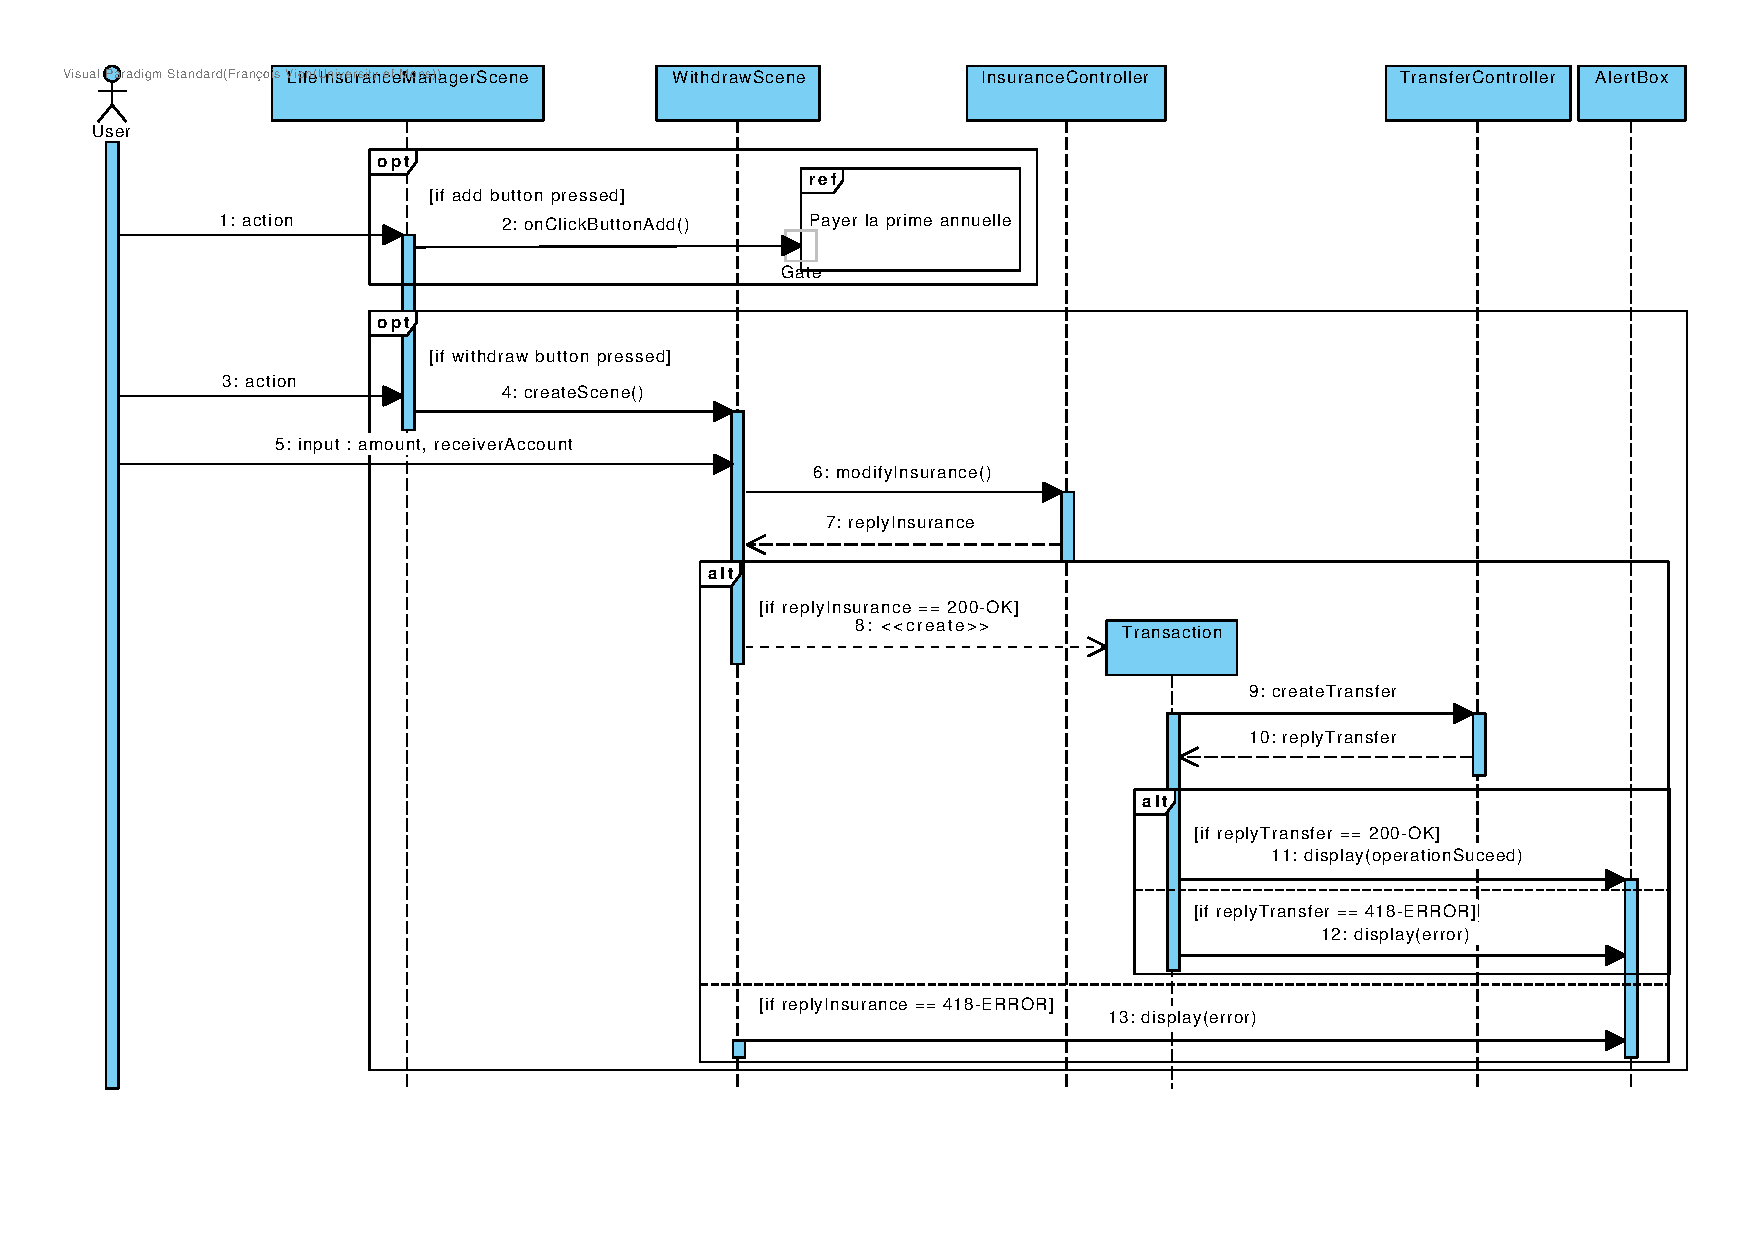
\includegraphics[width=\linewidth]{img/Gérer le montant sur une assurance.pdf}
    }
    \caption{Diagramme de séquence du use case "Gérer le montant sur une assurance"}
    \end{figure}

\paragraph{}On peut gérer le montant sur une assurance seulement pour les assurances vies. Cela se fait via un ajout ou un retrait d’argent. Si l’utilisateur clique sur le bouton d’ajout (1), il est redirigé vers le payement d’une prime (2) déjà décrite dans ce rapport. Si il clique sur le bouton de retrait (3), une scene est créée (4) dans laquelle l’utilisateur rentrera le montant qu’il souhaite retirer ainsi que le compte sur lequel il compte le recevoir (5). La scene fait ensuite un appel à l’API pour modifier l’assurance (6), celle-ci renvoie une réponse (7). Si la réponse est bonne, alors un objet Transaction est créé (8). Celui-ci va faire un appel à l’API pour créer un transfert (9) et recevoir une réponse de celle-ci (10). Si cette réponse est bonne, alors une fenêtre affichera que l’opération s’est effectuée avec succes. Si l’une des deux réponse est mauvase, une fenêtre affichera qu’il y a eu une erreur.

\end{document}